\documentclass[12pt,letterpaper]{article}

%%%%%%%%%%%%%%%%%%%%%%%%%%%%%%%%%%%%%%%%%%%%%%%%%

\usepackage{amsmath}
\usepackage{amssymb}
\usepackage{amsfonts}
\usepackage{array}
\usepackage{longtable}

\usepackage{lscape}
\usepackage{graphicx} 
\usepackage{rotating}

\usepackage{setspace}

%\usepackage{natbib}
\usepackage{multicol}
\pagestyle{empty}

%\bibpunct{(}{)}{;}{a}{,}{,}

%%%%%%%%%%%%%%%%%%%%%%%%%%%%%%%%%%%%%%%%%%%%%%%%%
%\usepackage{fullpage}

\topmargin 0pt
\advance \topmargin by -\headheight
\advance \topmargin by -\headsep
     
\textheight 8.9in
     
\oddsidemargin 0pt
\evensidemargin \oddsidemargin
\marginparwidth 0.5in
     
\textwidth 6.5in
%%%%%%%%%%%%%%%%%%%%%%%%%%%%%%%%%%%%%%%%%%%%%%%%%


\title{Eye Gaze Tracking using Eigen-eyes and Support Vector Machines}
\author{Mohammed Shoaib and Shreshth Singhal}
\date{January 17, 2012}

\begin{document}

\maketitle

\setstretch{1}

\begin{multicols}{2}algorithmic

\begin{abstract}
Human eye gaze tracking is an important problem with great potential in HCI. We created a robust but slow
eye tracker using correlation-based techniques. We then built gaze-tracking mechanisms on top of this.
Our approach to detect gaze direction was two-pronged: one using principal component analysis ('Eigen-eyes')
and one using support vector machines. The accuracy of these methods was measured to peak around 60-62\%.

\end{abstract}

%%%%%%%%%%%%%%%%%%%%%%%%%%%%%%%%%%%%%%%%%%%%%%%%%

\section{Introduction}
\label{scn:intro}

Eye gaze tracking means detecting the direction of line-of-sight of a person. Effective tracking of a 
person's gaze allows us to find out where their attention is focused. This valuable information can be 
leveraged in many ways. It can lead to new and potentially powerful human-computer interfaces, not only 
in theoretical systems and research, but in consumer applications. For example, a person could control 
the mouse on their computer using their gaze, allowing for quicker and more natural interaction. 
Consumer appliances like TVs could be equipped with simple cameras to perform basic tasks like turning
on or changing a channel based on a person's gaze. There have been forays in using gaze-tracking in 
museums to display information about the objects that the person is looking at\cite{museum}. The application 
which motivated this project was that of using a person's gaze as a cue to scroll through documents while 
reading them (when the user reaches the end of a page, the document auto-scrolls to the next page).

There are of course, intrusive, active methods of detecting eye gaze. One can easily attach probes 
around a person's eye to detect motion and derive the gaze from this - in fact this was a common method 
in earlier gaze trackers\cite{eyewriter}. There are also active methods which project infrared or 
near-infrared light onto the scene and detect the light reflected from the user's pupil as a bright spot.
The line-of-sight can then be gauged from this\cite{IR-tracking}\cite{starburst}.

We feel, for such a tracker to be a viable option in consumer applications, the goal must be to create 
a robust, non-invasive gaze tracker that works using simple cameras without needing any other active
assistance. There has been considerable research into developing such schemes. A very interesting method
exploits another vision problem - that of detecting head pose cues. This scheme uses a hybrid mechanism 
whereby the head pose and gaze are tracked independently using relatively weak trackers, and are then used 
mutually reinforce each other on successive iterations of the trackers\cite{synergetic-tracker}. Another 
very robust method is that of pupil center corneal reflection (PCCR). This method uses the 'glint' that 
appears on the cornea when a video is taken of the eye under sufficient light\cite{pccr-naive}. The naive
PCCR method has its drawbacks though, most notably its poor performance under significant head movement.
To allow for this, there is also a PCCR hybrid that allows for dynamic head movement compensation and 
works more robustly\cite{pccr-dynamic}.

%%%%%%%%%%%%%%%%%%%%%%%%%%%%%%%%%%%%%%%%%%%%%%%%%

\section{Goals and Challenges}
\label{scn:goals}

Our goals in this project were more modest than creating a robust eye-gaze tracker that works
perfectly even with considerable head movement. Our end goal was to design a system that would detect the
direction of a person's gaze with decent accuracy. However, before tackling the eye gaze problem, we need
to deal with tracking the eye. We need a method that can segment out the eye in a given set of video 
frames. Once we have the segmented eye, we need to extract the gaze information from it. 

There are numerous challenges that occur simply because of the way the problem is formulated. Chief amongst 
these is the problem of dealing with head movement. This can be dealt with in the earlier eye tracking step 
more easily since it is relatively easy to segment out the eye as long as it is visible in the video.
However, if we do this, then in the later stage, when we are trying to find the gaze direction, we have
no information about the depth and orientation of the eye with respect to the camera. This limits our
gaze tracking algorithms to those that work independent of knowledge about the eye's position. We can only
use the image of the eye and how the pupil is displaced. Intuitively, from the perspective of human vision,
this information is enough to figure out a person's line-of-sight. In fact, this is all the information 
that humans use to tell where a person is looking. Alternatively, if we wish to use the extra positional 
information, we can use more complicated mechanisms to allow for head movement as seen in \cite{pccr-dynamic}.

Another issue that arises is that of lighting - what if the image of the eye isn't bright enough to
glean any information from? Unfortunately, this can only be dealt with by artificially increasing the
light in the scene. 

%%%%%%%%%%%%%%%%%%%%%%%%%%%%%%%%%%%%%%%%%%%%%%%%%

\section{Eye tracking}
\label{scn:eyetrack}

The first step is to acquire frames from the video capture device separated by an appropriate amount of 
time. The time lag between frames mainly depends on the application. The time lag should be enough that
we don't get swamped with too much redundant image data. On the other hand, the frames need to be close 
together in time so that we don't end up missing any visual cues that the application may depend on (such 
as blinks or visual gestures). In our algorithm, there is an initial calibration step where the user must 
crop out the portion of any single frame that corresponds to their eye(s). This cropped out eye serves as
a template for the eye segmentation algorithm. 

For all the video frames, we compute the correlation coefficients between the template and all possible 
bounding boxes of the size of the template in the frame. The bounding box that gives the maximum 
correlation is the region where the eye is most likely to be. If the correlation coefficient at this point
has a value greater than a suitably chosen threshold value, we can assume with some confidence that it is
indeed the eye in that frame. Note that this threshold should be large enough to not allow false positives. 
On the other hand, it should not be so high that it doesn't allow for the expected variation in the way 
the eye looks from frame to frame.

%%%%%%%%%%%%%%%%%%%%%%%%%%%%%%%%%%%%%%%%%%%%%%%%%

\section{Gaze tracking}
\label{scn:gazetrack}

Once we have acquired the images of the eye from all the required video frames, we need to extract 
information about the gaze in each of them. At this point, as we mentioned before, we have no positional
information about the camera and the eye. All we have are the images of the eye themselves. To 
extract something useful out of these images, we need to compare them with 'canonical' images of the eye
pointing in known directions. We can then compare our test images with these known images to figure out
gaze direction. The term term 'compare' is somewhat loosely defined here. We will see further on
what techniques are actually used to do this. 

Note that this method limits us to only a fixed number of possible gaze directions, i.e. we have to
quantize the space of gaze directions down to a bounded set that we can reasonably train our algorithm 
on. We have chosen 9 possible gaze directions in our implementation. Also, note that the calibration 
images will be most effective if they are of the user's eyes; however, if we subtract colour information, 
any person's eye will work relatively well. 

With the test images and the training images that we have now, we use one of two techniques to find their
correlation:

\subsection{Eigen-eyes}
\label{scn:eigeneyes}

Once we have the training images and the images of the eye from video, we can use singular value 
decomposition (SVD) and principal components analysis (PCA) in a variant of the well-known eigen-faces 
algorithm. First off, we compute the average eye image and subtract it out from all the training images.
We then perform SVD on these normalized images to get the principal components of variation of the eye.
We can also compute the weights of these training images relative to their principal components (i.e. the
projections onto principal component axes).

Similarly, we normalize the test images from video, relative to the average eye. We then compute their
weights relative to the principal components (similar to above). Now, given the weights of all test
and training images relative to principal components, we can find the best match of each test image from
all the given training images. Our algorithm simply computes the euclidean difference between the two 
weights. The training image that minimizes this distance for a given test image is said to be the closest 
match for that test image. 

We know the direction of gaze of the eye in the best match training image. We can assume that the 
eye in the corresponding test image is also pointed in that direction.

\subsection{Support Vector Machines}
\label{scn:svm}

An alternative method for gaze tracking is using the SVM recognition technique. SVM is a basic recognition
and classification technique that, at its simplest, is use to classify data into one of two classes, after
being appropriately trained by examples of both classes. Theoretically, it achieves this by finding the
hyperplane that separates the points corresponding to members of the two classes in a way that maximizes
the margin between the hyperplane and members of the two sets. This problem reduces to a minimization 
problem subject to constraints of correctly classifying the data. From this programming problem, we learn
the support vectors (that lie on the margin around the hyperplane). The hyperplane may sometimes 
need to be in a higher-dimension to correctly classify all data points. To avoid the transformation 
to higher dimensions, we can use kernel functions. These are nonlinear boundaries that work similar to 
how a linear boundary would in higher dimensions.

While the basic form of SVM is a binary classifier, it can be expanded by two different methods to become
a multi-class classifier. The first, called 'one against all' trains by learning a binary SVM for one class
versus a class that is the union of all the others. It classifies test data by applying such an SVM for
each class. The class that returns the best matching value is the one that is deemed correct. The second
method, called 'one against one' trains by learning an SVM for each pair of classes. To classify test
data, we apply all these SVMs. The class that the test data is classified into the most is considered to 
be the correct class.

In our algorithm, we used a third-party SVM toolbox \cite{SVM-KMToolbox} to perform multi-class 
classification amongst our gaze classes. 

%%%%%%%%%%%%%%%%%%%%%%%%%%%%%%%%%%%%%%%%%%%%%%%%%

\end{multicols}

\begin{figure}[h]
\centering
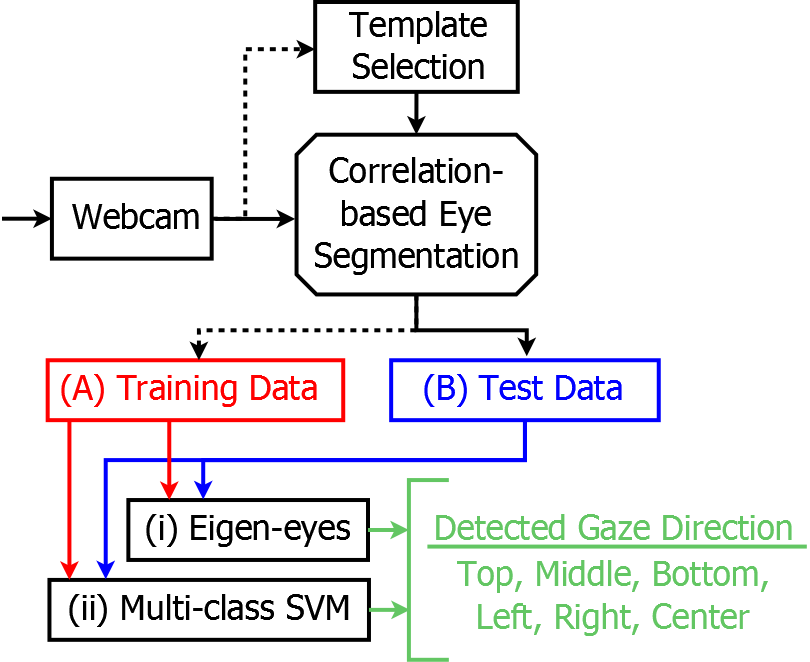
\includegraphics[width=130mm,height=90mm]{algo.png}
\caption{Flow-chart of the algorithm. Dashed lines are one-time training steps. Solid lines are continuous
stream of data}
\end{figure}

\newpage

\begin{multicols}{2}

%%%%%%%%%%%%%%%%%%%%%%%%%%%%%%%%%%%%%%%%%%%%%%%%%

\section{Results}
\label{scn:results}

\subsection{Eye tracking}
\label{scn:results-eyetrack}

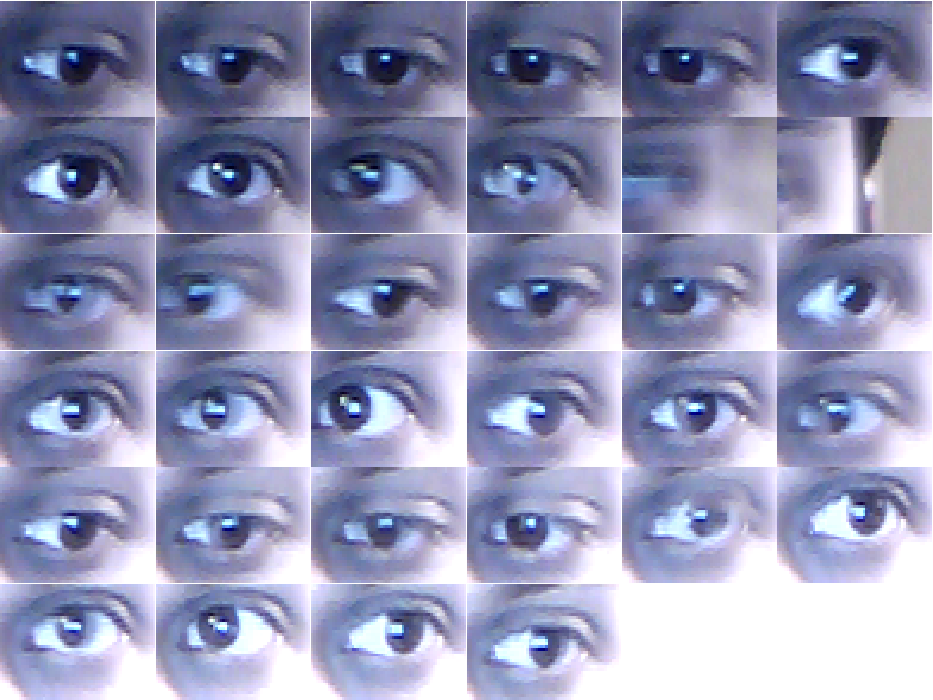
\includegraphics[width=80mm,height=100mm]{segmentEyes.png}

caption{Figure 2: Results of eye segmentation}

\medskip
The above image shows the result of the eye segmentation algorithm for a general trial run. The user in
front of the camera moved his eyes all around the screen. After picking the template, the bounding boxes
in all the frames are correlated to find the best match with the eye. As can be seen in this, the 
algorithm does quite a good job. In all but one frame (plus another hazy frame), the correct eye position 
has been found; in fact the bounding box is found such that the eye is centered in most of these images. 
This provides a fairly uniform dataset for the gaze tracker to work with. 

The cons of this approach is that the segmentation step is quite slow. It can take a upto 2 minutes or so
to segment the eye from 50 test frames. Also, if the user picks a larger template, then we end up with more 
information than necessary. In fact, in the gaze tracking step, if there is too much information outside 
the eye itself, it can be detrimental as it reduces the importance of the eye and the direction where
the eye is pointing. This can lead to a lot of false positives in gaze tracking, since images will be
matched to the wrong set. 

\subsection{Eigen-eyes}
\label{scn:results-eigeneyes}

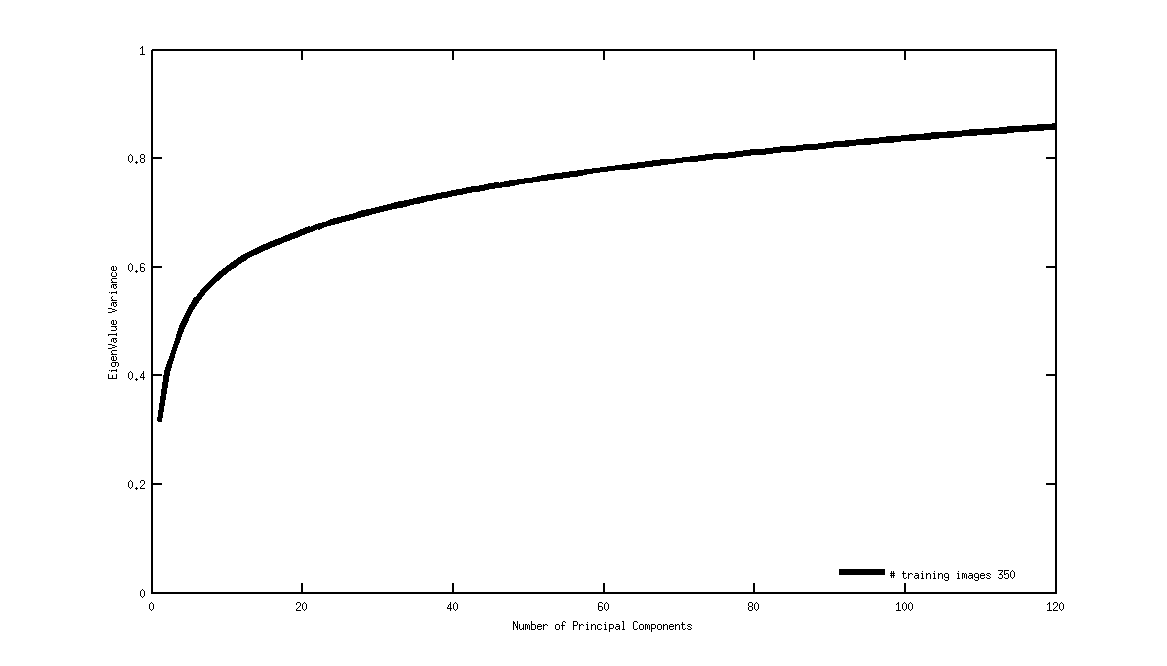
\includegraphics[width=10cm]{eigenValueVariance.png}

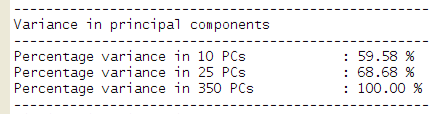
\includegraphics[width=10cm]{eigenValueVariance2.png}

\small Figure 3: Variance in eigenvalues as a function of number of principal components
(units on the X-axis are in increments of 20).

\medskip
When using the Eigen-eyes algorithm, we can see that the variation in the eigenvalues plateaus after 
15-20 distinct principal components are chosen. The number of principal components chosen to run the 
algorithm is an important consideration. More principal components mean we get more precise reconstruction
and matching of the test images; however, this comes at the cost of extra computation. As we can see from
the above graph, the law of diminishing returns applies and we don't get much added benefit in going beyond
20 eigen-eyes.
\newpage
When using 25 eigen-eyes, we get the following results:

\end{multicols}

\begin{figure}[h]
%\centering
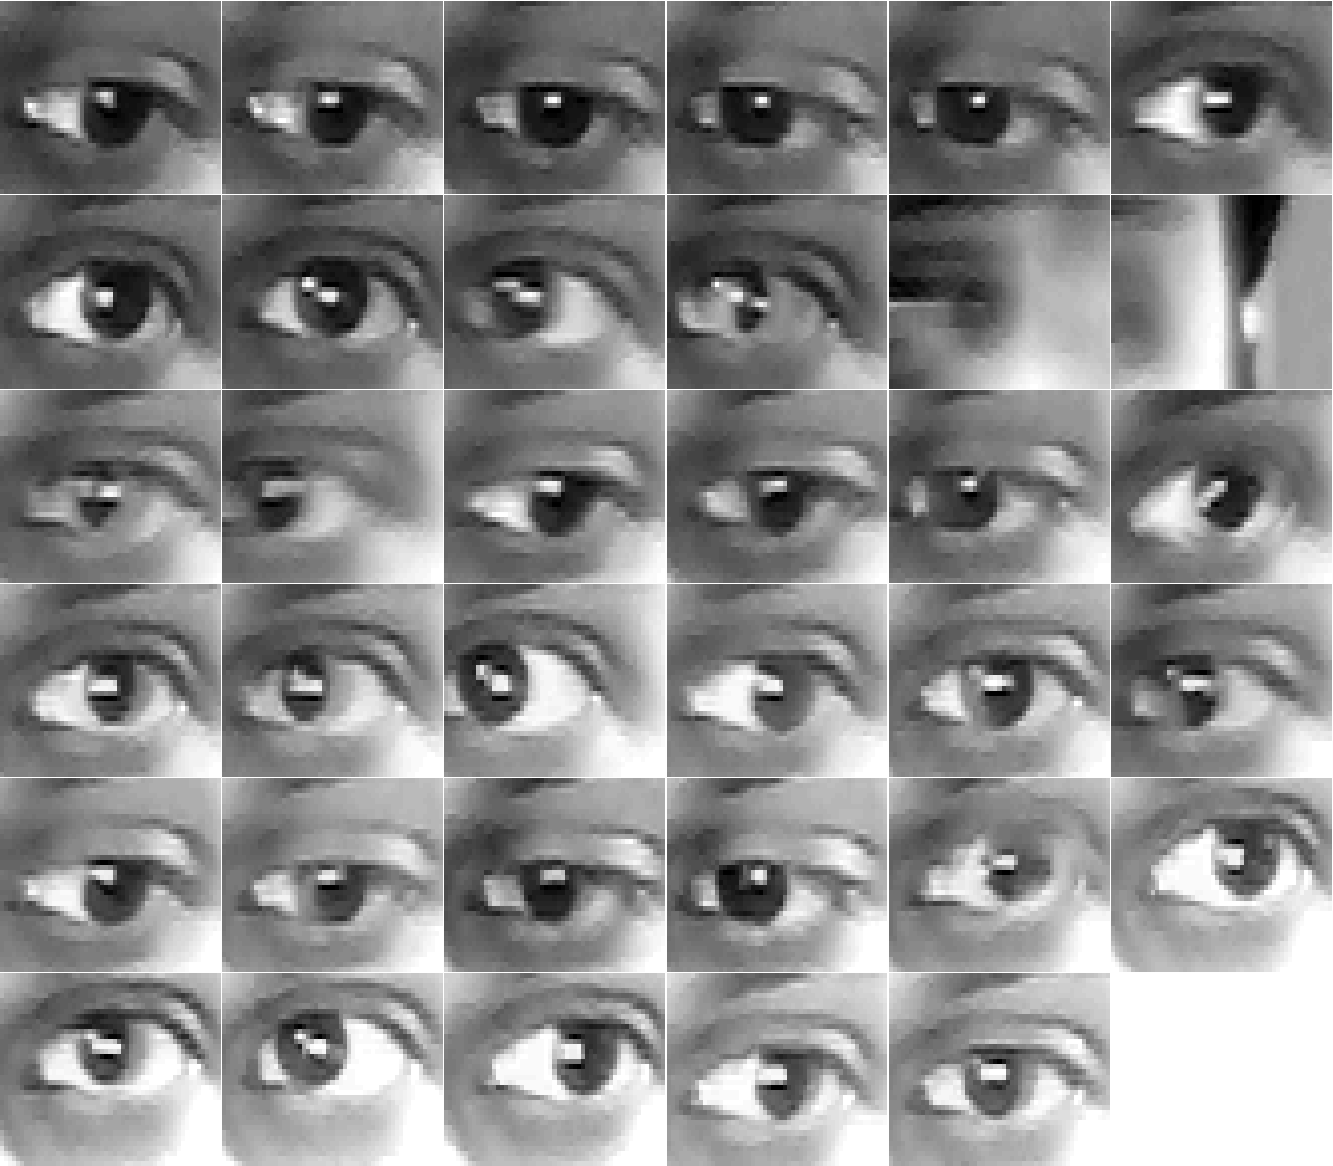
\includegraphics[width=79mm,height=95mm]{testImg.png}
\hfill
%\centering
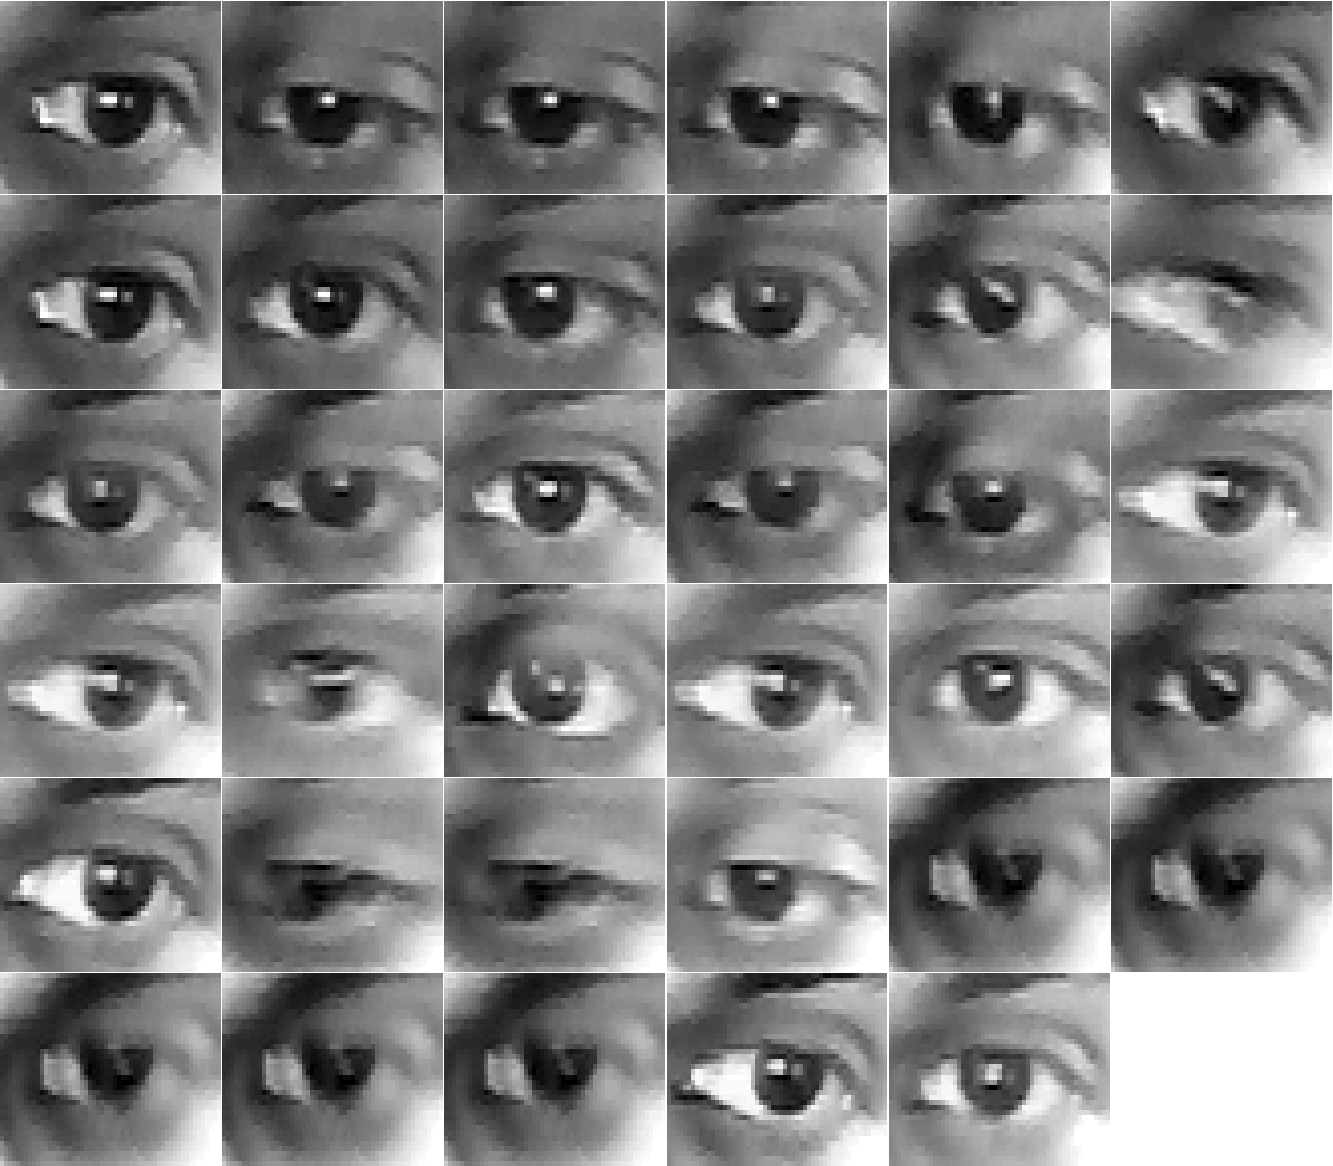
\includegraphics[width=79mm,height=95mm]{matchImg.png}

\small \quad\qquad\qquad\qquad\qquad Figure 4: Test images \qquad\qquad\qquad
\small Figure 5: Corresponding best-match training images
\end{figure}

\begin{figure}[h]
\centering
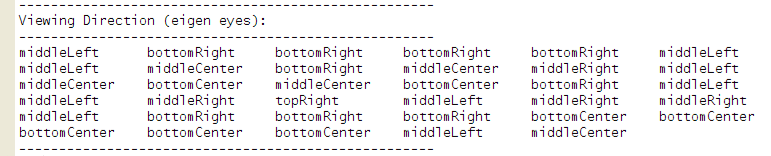
\includegraphics[width=170mm,height=50mm]{viewingDir.png}

\small Figure 6: Corresponding best-match gaze direction
\end{figure}

This gives 21 correct out of 35, a success rate of 60\%.

\newpage

Using 15 eigenvalues instead, we get the following:

\begin{figure}[h]
%\centering
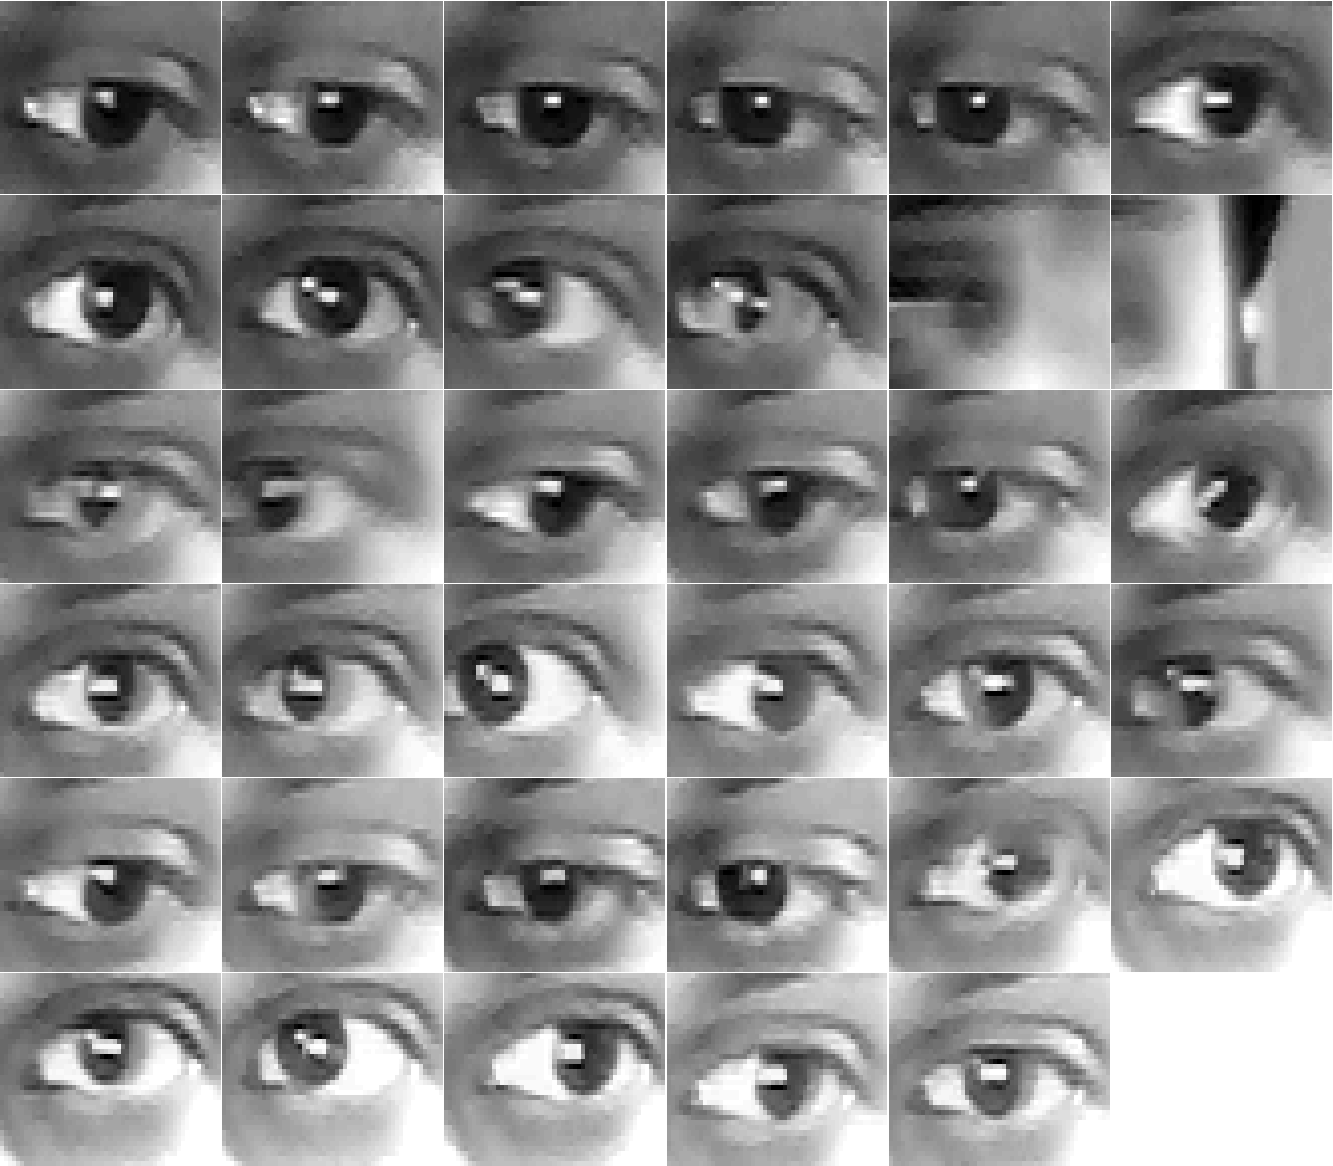
\includegraphics[width=79mm,height=95mm]{testImg2.png}
\hfill
%\centering
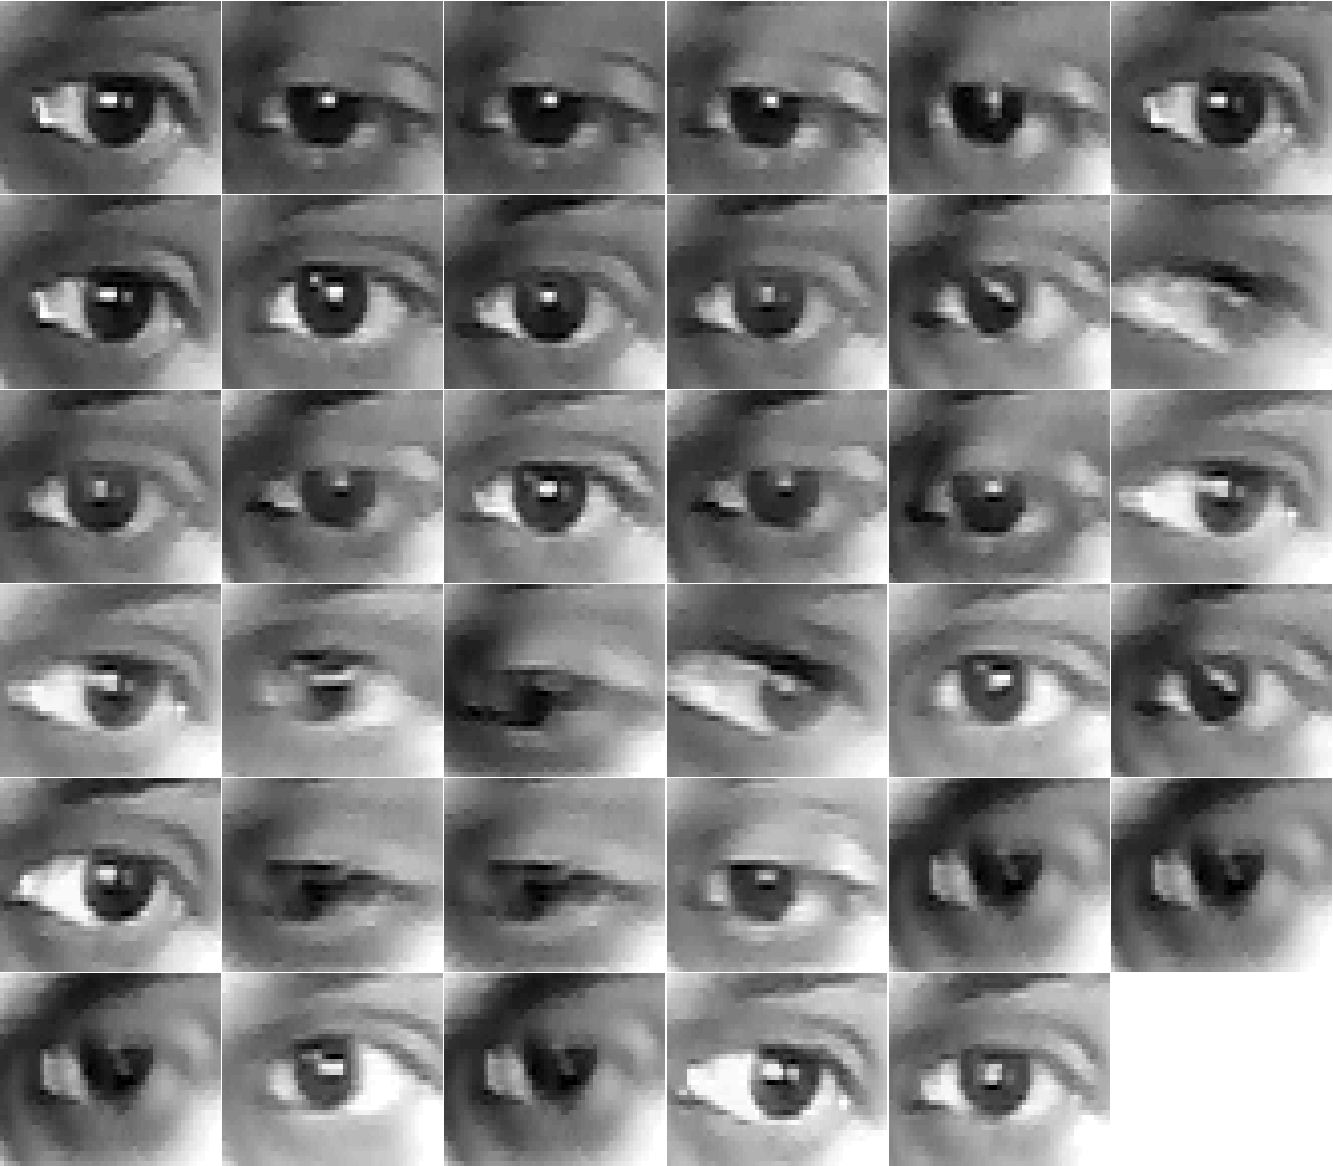
\includegraphics[width=79mm,height=95mm]{matchImg2.png}

\small \quad\qquad\qquad\qquad\qquad Figure 7: Test images \qquad\qquad\qquad
\small Figure 8: Corresponding best-match training images
\end{figure}

\begin{figure}[h]
\centering
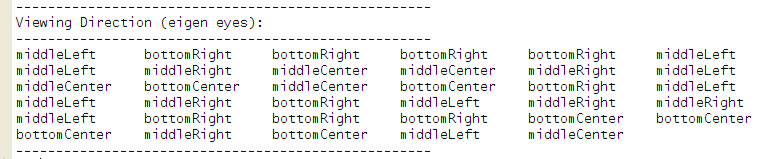
\includegraphics[width=170mm,height=50mm]{viewingDir2.png}

\small Figure 9: Corresponding best-match gaze direction
\end{figure}

This gives 18/35 correct, that is about 51\% correct.

\newpage

Using 5 eigenvalues, we get:

\begin{figure}[h]
%\centering
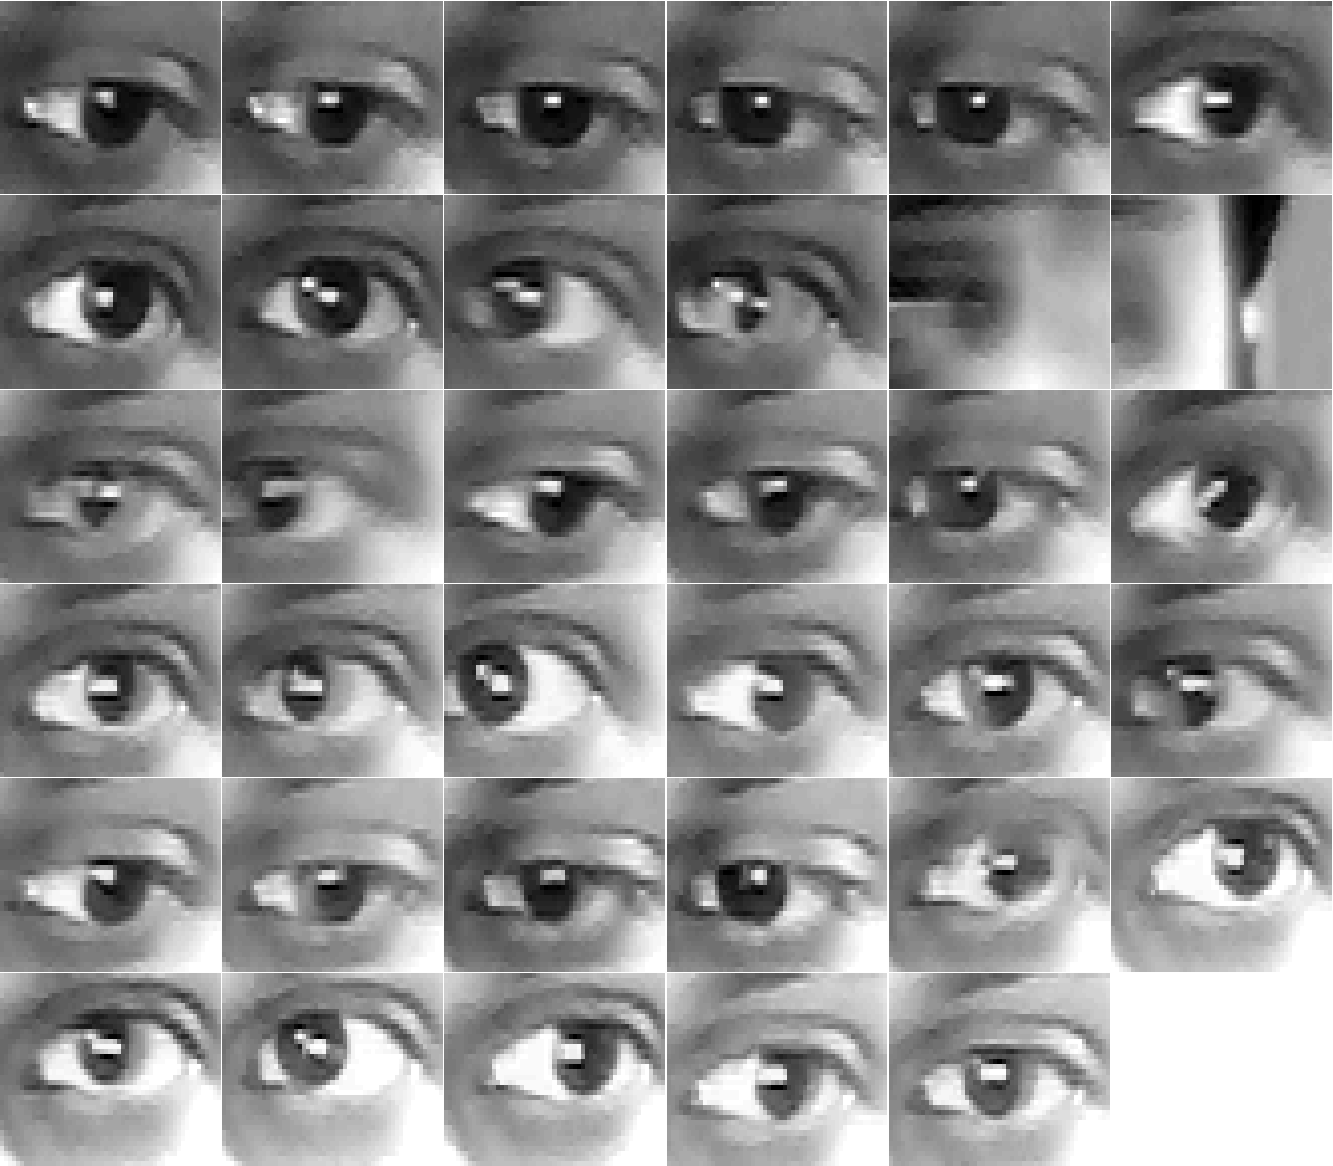
\includegraphics[width=79mm,height=95mm]{testImg3.png}
\hfill
%\centering
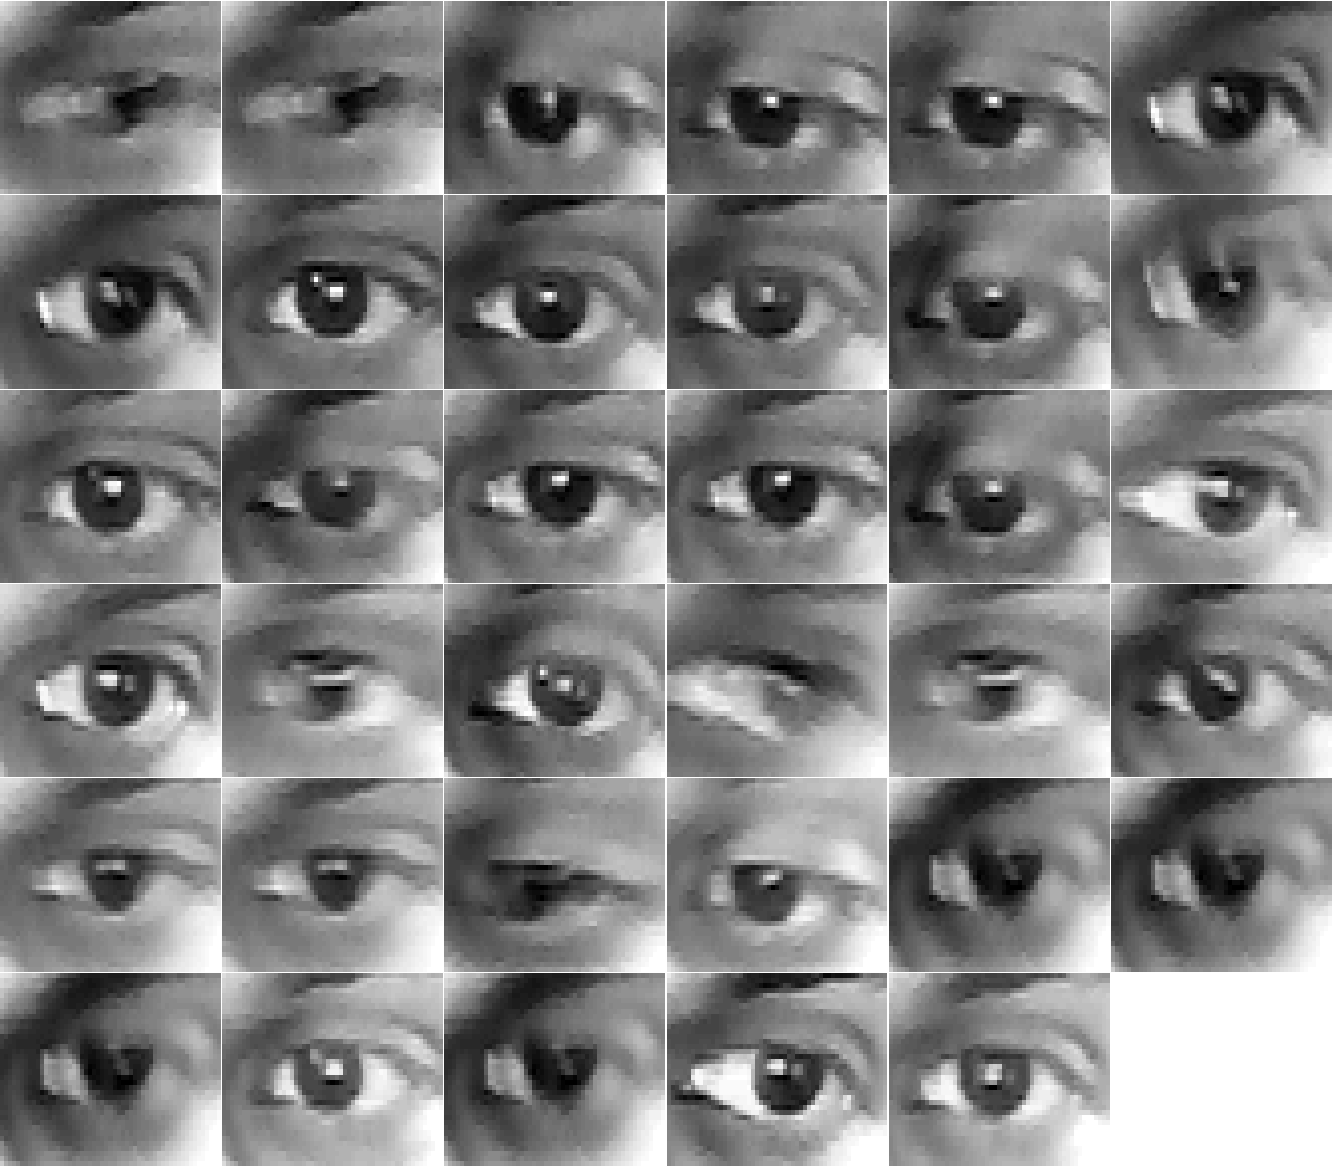
\includegraphics[width=79mm,height=95mm]{matchImg3.png}

\small \quad\qquad\qquad\qquad\qquad Figure 10: Test images \qquad\qquad\qquad
\small Figure 11: Corresponding best-match training images
\end{figure}

\begin{figure}[h]
\centering
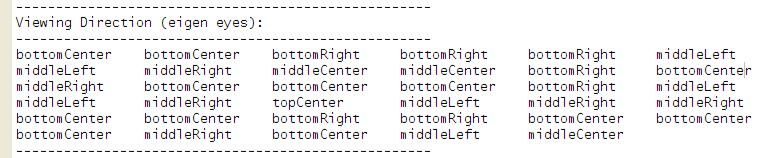
\includegraphics[width=170mm,height=50mm]{viewingDir3.png}

\small Figure 12: Corresponding best-match gaze direction
\end{figure}

This gives 13 out of 35 correct, for a correctness of about 37\%.

\newpage For the curious, here are the eigen-eyes themselves:
\begin{figure}[h]
\centering
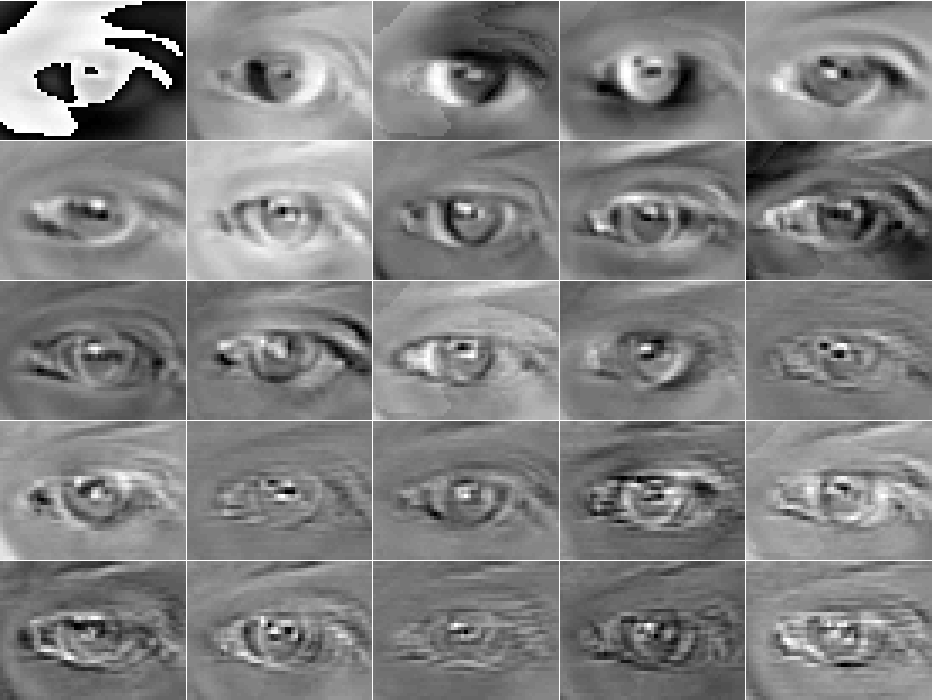
\includegraphics[width=10cm]{eigenEyes.png}

\small Figure 13: Eigen-eyes
\end{figure}

And the following are the reconstructed eyes:

\begin{figure}[h]
\centering
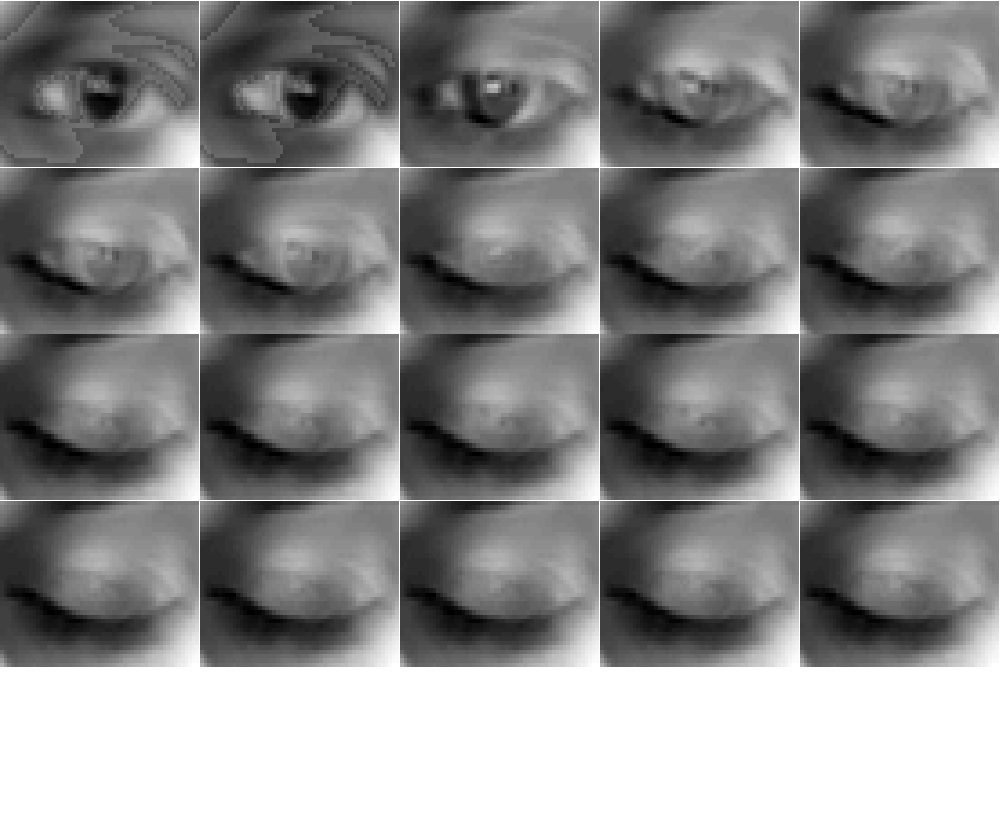
\includegraphics[width=8.5cm]{reconEye.png}

\small Figure 14: Reconstructed eyes
\end{figure}

Hence, our eigen-eyes method works fairly well in tracking the gaze. It is also apparent that the number
of principal components is a critical parameter in using this method successfully. The more principal
components we can use, the greater the number of choices we have to find matchings from, and hence the 
better job we can do. At the same time, the effect of increasing the number of principal components 
plateaus out after about 15-20 principal components, so there is not much reason to optimize after this 
point.

\subsection{SVM}
\label{scn:results-svm}

Here are the results of using SVM with the one-versus-one multi-class method and a polynomial kernel
function of degree 1:

\begin{figure}[h]
\centering
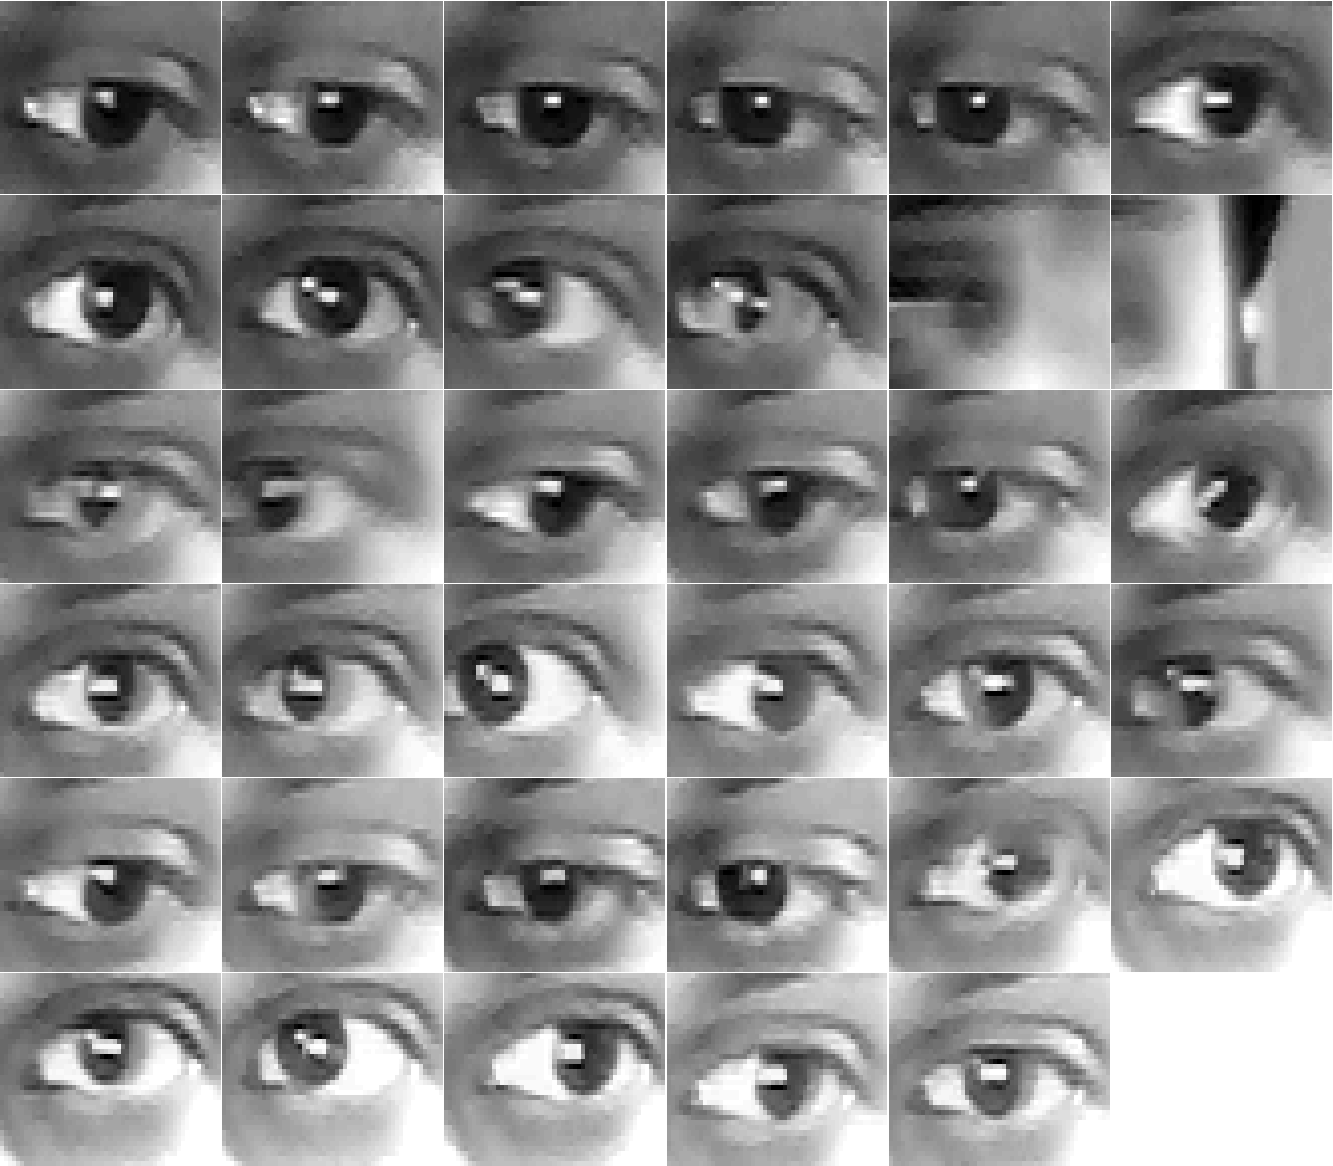
\includegraphics[width=120mm,height=95mm]{testImg3.png}

\small Figure 15: Test images
\end{figure}

\begin{figure}[h]
\centering
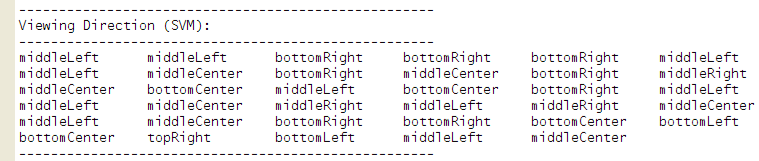
\includegraphics[width=170mm,height=50mm]{viewingDir4.png}

\small Figure 16: Corresponding best-match gaze direction
\end{figure}

This gives 22 correct out of 35, for a correctness of about 62.8\%. It is quite interesting to note that
this linear polynomial function works quite well, but any polynomial of greater degree fails entirely
and just classifies all objects to the same class. This is quite strange behaviour. One could expect a 
polynomial function of higher degree with a gentle curve (low gradient) could approximate quite well, the
job of a linear function. Maybe this arises because of the way the data points are apparently mapped
to the higher dimension, causing them to become clumped together.

\newpage

On using one-versus-all classifier, with the same polynomial kernel, we get:

\begin{figure}[h]
\centering
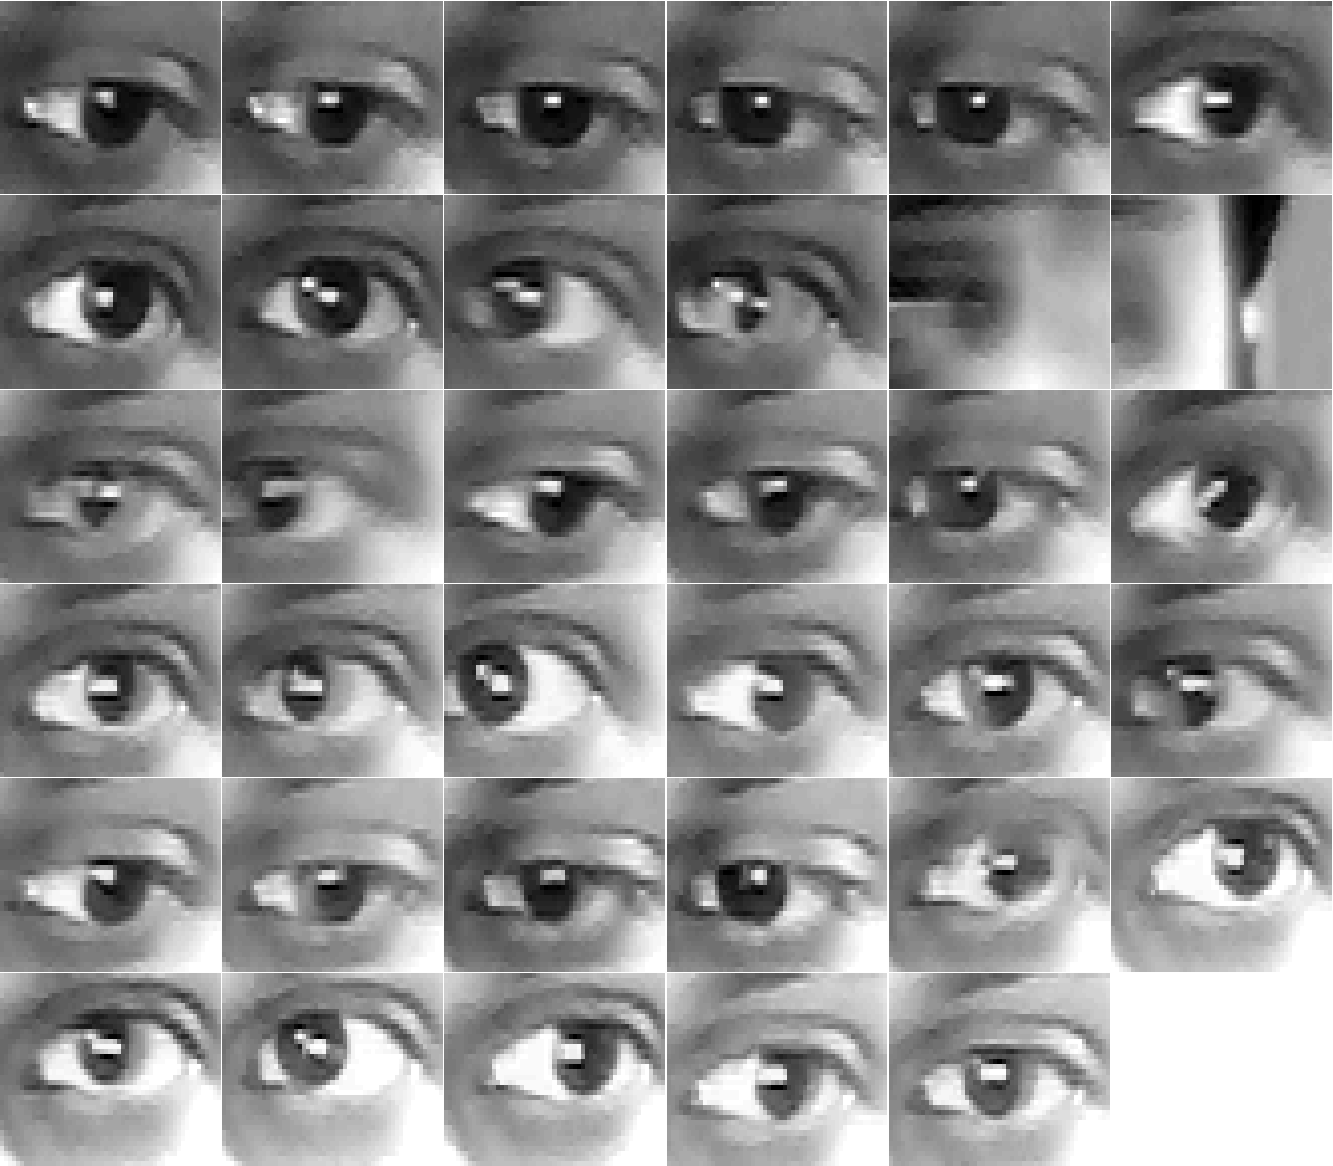
\includegraphics[width=120mm,height=95mm]{testImg3.png}

\small Figure 17: Test images
\end{figure}

\begin{figure}[h]
\centering
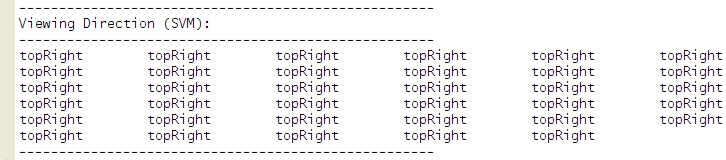
\includegraphics[width=170mm,height=50mm]{viewingDir5.png}

\small Figure 18: Corresponding best-match gaze direction
\end{figure}

Here, there is obviously something wrong with the classification process. The SVM classifier has lumped
everything together, and simply labelled everything to be the same. The reason behind this could be that
the space for training an SVM with all the classes (one-versus-all) may be a lot more complex than one 
where we are only dealing with two classes (one-versus-one). Hence, the kernel function which emulates the 
lift to higher dimensionality must be chosen correctly to account for this fact. With the toolbox that we
used, none of the given kernel functions actually worked in classifng the data. All of them had similar 
results to the above. We hope to tackle this befuddling problem in the future. 

\newpage

Here are the results of using SVM with the one-versus-one multi-class method and a homogeneous polynomial
kernel function of degree 1:

\begin{figure}[h]
\centering
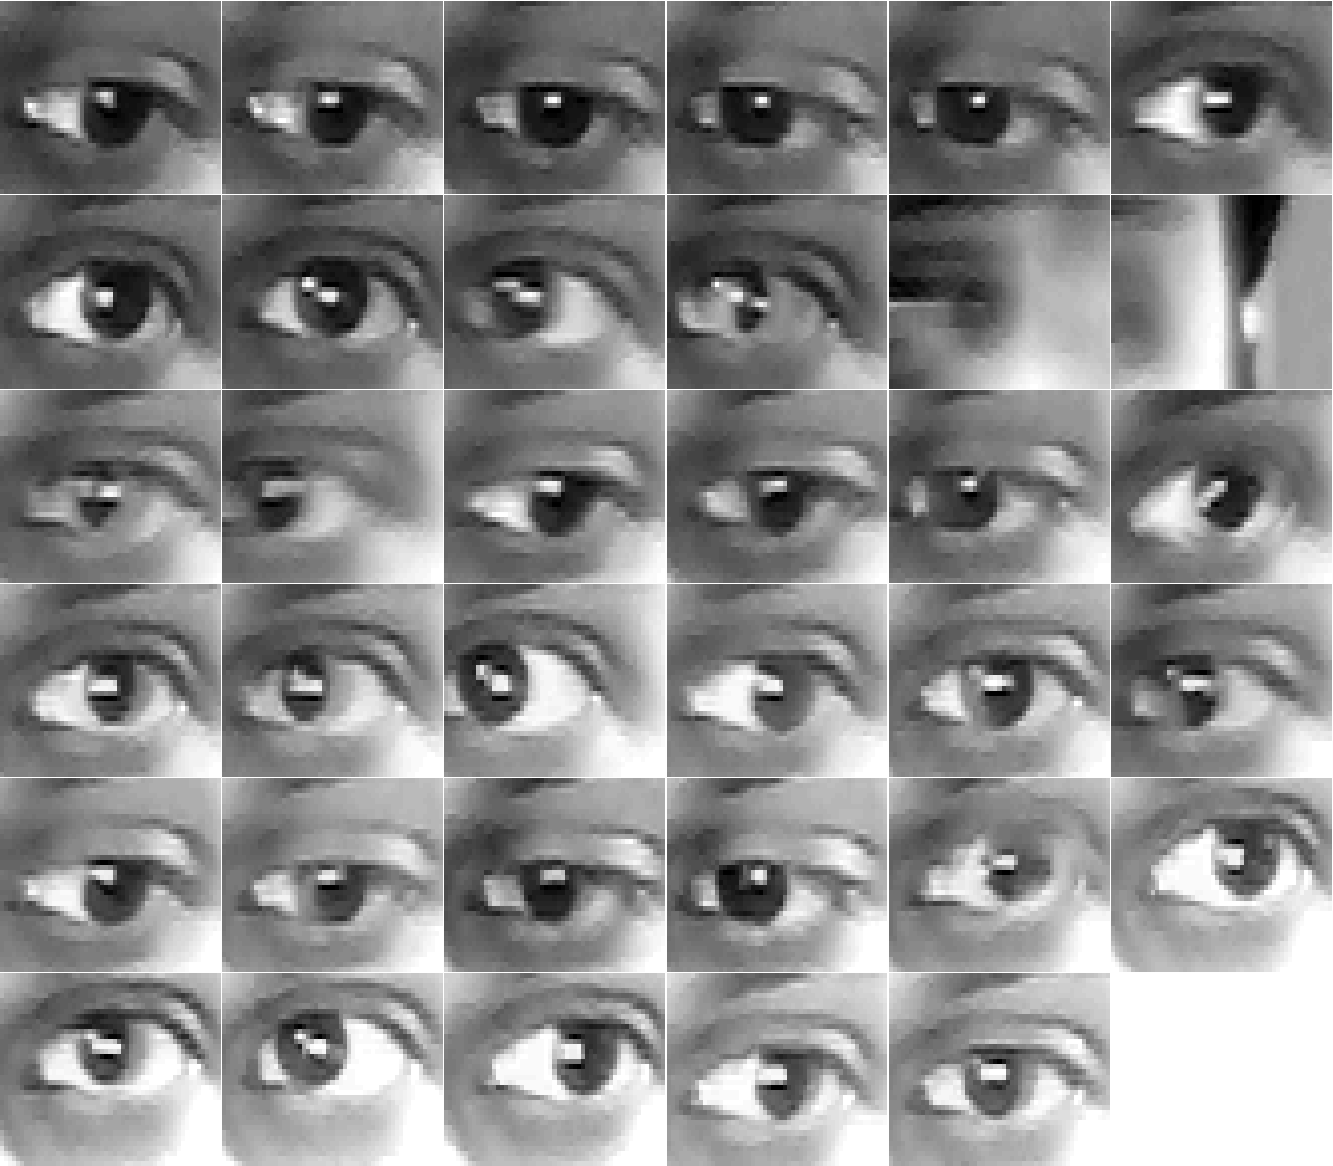
\includegraphics[width=120mm,height=95mm]{testImg3.png}

\small Figure 19: Test images
\end{figure}

\begin{figure}[h]
\centering
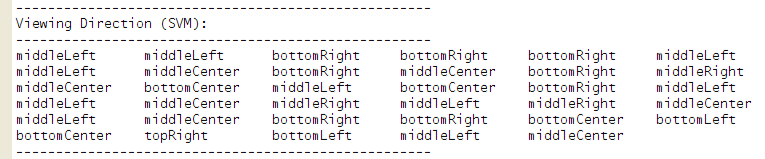
\includegraphics[width=170mm,height=50mm]{viewingDir6.png}

\small Figure 20: Corresponding best-match gaze direction
\end{figure}

This gives 22 correct out of 35, for a correctness of about 62.8\%. This function works quite similar to
the related simple polynomial kernel. It also shows similar gibberish results for higher degree functions.

Hence, the SVM classifier does quite well when we appropriately choose the method for doing multi-class 
classification. Also, the validity of the classification depends on the kernel function we use. 

\newpage

\begin{multicols}{2}

\subsection{Summary}
\label{scn:summary}

We have seen, therefore, that the eye segmentation method works slowly, but does quite a good job of
detecting the eye across frames, given a suitable template. On the contrary, the gaze tracking methods 
work much faster, but aren't nearly as robust. At their most optimized states, they both achieve
similar levels of success (around 60\% correct classification). Choosing the parameters is important to 
reach this upper limit; for a lot of choices, the algorithms may just not work at all. 



%%%%%%%%%%%%%%%%%%%%%%%%%%%%%%%%%%%%%%%%%%%%%%%%%

\section{Issues and further work}
\label{scn:issues}

While this gaze tracker is an interesting theoretical project, our motivation was to integrate it without
document readers to allow for an auto-scrolling application. As of now, our algorithm is not robust enough
to allow for this. We have identified the following issues and potential solutions to them for future work:

\begin{enumerate}
\item
The gaze tracking algorithm isn't extremely accurate. For a real system, we would need the tracker to work
extremely accurately so that the user doesn't have to wait forever for the algorithm to register their
cues. We can try to reduce the amount of redundant information the tracker gets, by cropping out all of the
eye image except the eye part itself using some variant of circle detector. This will help us get the 
necessary information - the direction of the eyeball - without other distracting information that may be
leading to false positives. We can also look further into other, more robust algorithms like the hybrid 
PCCR algorithm\cite{pccr-dynamic}. This algorithm will further resolve potential issues about invariance 
to scale and head movement.
\item 
The eye-segmentation algorithm is relatively slow, since it is correlation based (even though it performs 
remarkably well). We tried using alternative approaches such as Hough transforms, but those were slow as 
well. We will have to research further and look for faster and equally robust methods, possibly using a
variety of less complex algorithms, like edge detectors. 
\end{enumerate}

\end{multicols}

%%%%%%%%%%%%%%%%%%%%%%%%%%%%%%%%%%%%%%%%%%%%%%%%%

\newpage
\bibliographystyle{plain}
\bibliography{report-bib.bib}

\end{document}